\title{2017 年高考数学 全国III卷-理科}
\date{}
\maketitle

\section*{一、单项选择题}
本题共12小题，每小题5分，共60分。在每小题给出的四个选项中，只有一项是符合题目要求的。

\begin{question}[points=5]
已知集合$A=\{(x,y)|x^2+y^2=1\}$，$B=\{(x,y)|y=x\}$，则$A\cap B$中元素的个数为（ ）
\begin{choices}
  \item $3$
  \item $2$
  \item $1$
  \item $0$
\end{choices}
\begin{solution}
\textbf{答案：}$B$

\textbf{分析：}解不等式组求出元素的个数即可。

\textbf{详解：}由$\begin{cases} x^2+y^2=1 \\ y=x \end{cases}$，解得：$\begin{cases} x=\frac{\sqrt{2}}{2} \\ y=\frac{\sqrt{2}}{2} \end{cases}$或$\begin{cases} x=-\frac{\sqrt{2}}{2} \\ y=-\frac{\sqrt{2}}{2} \end{cases}$，∴$A\cap B$的元素的个数是2个。故选B。
\end{solution}
\end{question}

\begin{question}[points=5]
设复数$z$满足$(1+i)z=2i$，则$|z|=$（ ）
\begin{choices}
  \item $\frac{1}{2}$
  \item $\frac{\sqrt{2}}{2}$
  \item $\sqrt{2}$
  \item $2$
\end{choices}
\begin{solution}
\textbf{答案：}$C$

\textbf{分析：}利用复数的运算法则、模的计算公式即可得出。

\textbf{详解：}∵$(1+i)z=2i$，∴$(1-i)(1+i)z=2i(1-i)$，$z=i+1$。则$|z|=\sqrt{2}$。故选C。
\end{solution}
\end{question}

\begin{question}[points=5]
某城市为了解游客人数的变化规律，提高旅游服务质量，收集并整理了2014年1月至2016年12月期间月接待游客量（单位：万人）的数据，绘制了下面的折线图。根据该折线图，下列结论错误的是（ ）

\begin{center}
  
\includegraphics[width=.38\linewidth]{question-3-1.jpg}
\end{center}
\begin{choices}
  \item $A$．月接待游客量逐月增加
  \item $B$．年接待游客量逐年增加
  \item $C$．各年的月接待游客量高峰期大致在7，8月
  \item $D$．各年1月至6月的月接待游客量相对于7月至12月，波动性更小，变化比较平稳
\end{choices}
\begin{solution}
\textbf{答案：}$A$

\textbf{分析：}根据已知中2014年1月至2016年12月期间月接待游客量（单位：万人）的数据，逐一分析给定四个结论的正误，可得答案。

\textbf{详解：}由已有中2014年1月至2016年12月期间月接待游客量（单位：万人）的数据可得：月接待游客量逐月有增有减，故A错误；年接待游客量逐年增加，故B正确；各年的月接待游客量高峰期大致在7，8月，故C正确；各年1月至6月的月接待游客量相对于7月至12月，波动性更小，变化比较平稳，故D正确。故选A。
\end{solution}
\end{question}

\begin{question}[points=5]
$(x+y)(2x-y)^5$的展开式中的$x^3y^3$系数为（ ）
\begin{choices}
  \item $-80$
  \item $-40$
  \item $40$
  \item $80$
\end{choices}
\begin{solution}
\textbf{答案：}$C$

\textbf{分析：}$(2x-y)^5$的展开式的通项公式：$T_{r+1}=C_{5}^{r}(2x)^{5-r}(-y)^r=2^{5-r}(-1)^r C_{5}^{r}x^{5-r}y^r$。令$5-r=2$，$r=3$，解得$r=3$。令$5-r=3$，$r=2$，解得$r=2$。即可得出。

\textbf{详解：}$(2x-y)^5$的展开式的通项公式：$T_{r+1}=C_{5}^{r}(2x)^{5-r}(-y)^r=2^{5-r}(-1)^r C_{5}^{r}x^{5-r}y^r$。令$5-r=2$，$r=3$，解得$r=3$。令$5-r=3$，$r=2$，解得$r=2$。∴$(x+y)(2x-y)^5$的展开式中的$x^3y^3$系数$=2^2\times(-1)^3 C_{5}^{3}+2^3\times C_{5}^{2}=40$。故选C。
\end{solution}
\end{question}

\begin{question}[points=5]
已知双曲线$C:\frac{x^2}{a^2}-\frac{y^2}{b^2}=1$（$a>0$，$b>0$）的一条渐近线方程为$y=\frac{\sqrt{5}}{2}x$，且与椭圆$\frac{x^2}{12}+\frac{y^2}{3}=1$有公共焦点，则$C$的方程为（ ）
\begin{choices}
  \item $\frac{x^2}{8}-\frac{y^2}{10}=1$
  \item $\frac{x^2}{4}-\frac{y^2}{5}=1$
  \item $\frac{x^2}{5}-\frac{y^2}{4}=1$
  \item $\frac{x^2}{4}-\frac{y^2}{3}=1$
\end{choices}
\begin{solution}
\textbf{答案：}$B$

\textbf{分析：}求出椭圆的焦点坐标，得到双曲线的焦点坐标，利用双曲线的渐近线方程，求出双曲线实半轴与虚半轴的长，即可得到双曲线方程。

\textbf{详解：}椭圆$\frac{x^2}{12}+\frac{y^2}{3}=1$的焦点坐标$(\pm 3,0)$，则双曲线的焦点坐标为$(\pm 3,0)$，可得$c=3$。双曲线$C:\frac{x^2}{a^2}-\frac{y^2}{b^2}=1$（$a>0$，$b>0$）的一条渐近线方程为$y=\frac{\sqrt{5}}{2}x$，可得$\frac{b}{a}=\frac{\sqrt{5}}{2}$，即$\frac{b^2}{a^2}=\frac{5}{4}$，可得$\frac{c^2-a^2}{a^2}=\frac{5}{4}$，$\frac{9-a^2}{a^2}=\frac{5}{4}$，解得$a=2$，$b=\sqrt{5}$。所求的双曲线方程为：$\frac{x^2}{4}-\frac{y^2}{5}=1$。故选B。
\end{solution}
\end{question}

\begin{question}[points=5]
设函数$f(x)=\cos(x+\frac{\pi}{3})$，则下列结论错误的是（ ）
\begin{choices}
  \item $A$．$f(x)$的一个周期为$-2\pi$
  \item $B$．$y=f(x)$的图象关于直线$x=\frac{8\pi}{3}$对称
  \item $C$．$f(x+\pi)$的一个零点为$x=\frac{\pi}{6}$
  \item $D$．$f(x)$在$(\frac{\pi}{2},\pi)$单调递减
\end{choices}
\begin{solution}
\textbf{答案：}$D$

\textbf{分析：}根据三角函数的图象和性质分别进行判断即可。

\textbf{详解：}A．函数的周期为$2k\pi$，当$k=-1$时，周期$T=-2\pi$，故A正确。B．当$x=\frac{8\pi}{3}$时，$\cos(\frac{8\pi}{3}+\frac{\pi}{3})=\cos(3\pi)=-1$为最小值，此时$y=f(x)$的图象关于直线$x=\frac{8\pi}{3}$对称，故B正确。C．当$x=\frac{\pi}{6}$时，$f(\frac{\pi}{6}+\pi)=\cos(\frac{\pi}{6}+\pi+\frac{\pi}{3})=\cos\frac{3\pi}{2}=0$，则$f(x+\pi)$的一个零点为$x=\frac{\pi}{6}$，故C正确。D．当$\frac{\pi}{2}<x<\pi$时，$\frac{5\pi}{6}<x+\frac{\pi}{3}<\frac{4\pi}{3}$，此时函数$f(x)$不是单调函数，故D错误。故选D。
\end{solution}
\end{question}

\begin{question}[points=5]
执行如图的程序框图，为使输出$S$的值小于$91$，则输入的正整数$N$的最小值为（ ）

\begin{center}
  
\includegraphics[width=.38\linewidth]{question-7-1.jpg}
\end{center}
\begin{choices}
  \item $5$
  \item $4$
  \item $3$
  \item $2$
\end{choices}
\begin{solution}
\textbf{答案：}$D$

\textbf{分析：}通过模拟程序，可得到S的取值情况，进而可得结论。

\textbf{详解：}由题可知初始值$t=1$，$M=100$，$S=0$，要使输出$S$的值小于$91$，应满足“$t\le N$”，则进入循环体，从而$S=100$，$M=-10$，$t=2$，要使输出$S$的值小于$91$，应接着满足“$t\le N$”，则进入循环体，从而$S=90$，$M=1$，$t=3$，要使输出$S$的值小于$91$，应不满足“$t\le N$”，跳出循环体，此时$N$的最小值为$2$。故选D。
\end{solution}
\end{question}

\begin{question}[points=5]
已知圆柱的高为$1$，它的两个底面的圆周在直径为$2$的同一个球的球面上，则该圆柱的体积为（ ）
\begin{choices}
  \item $\pi$
  \item $\frac{3\pi}{4}$
  \item $\frac{\pi}{2}$
  \item $\frac{\pi}{4}$
\end{choices}
\begin{solution}
\textbf{答案：}$B$

\textbf{分析：}推导出该圆柱底面圆周半径$r=\sqrt{1^2-(\frac{1}{2})^2}=\frac{\sqrt{3}}{2}$，由此能求出该圆柱的体积。

\textbf{详解：}∵圆柱的高为$1$，它的两个底面的圆周在直径为$2$的同一个球的球面上，∴该圆柱底面圆周半径$r=\sqrt{1^2-(\frac{1}{2})^2}=\frac{\sqrt{3}}{2}$，∴该圆柱的体积：$V=Sh=\pi\times(\frac{\sqrt{3}}{2})^2\times1=\frac{3\pi}{4}$。故选B。
\end{solution}
\end{question}

\begin{question}[points=5]
等差数列$\{a_n\}$的首项为$1$，公差不为$0$．若$a_2$，$a_3$，$a_6$成等比数列，则$\{a_n\}$前$6$项的和为（ ）
\begin{choices}
  \item $-24$
  \item $-3$
  \item $3$
  \item $8$
\end{choices}
\begin{solution}
\textbf{答案：}$A$

\textbf{分析：}利用等差数列通项公式、等比数列性质列出方程，求出公差，由此能求出$\{a_n\}$前6项的和。

\textbf{详解：}∵等差数列$\{a_n\}$的首项为$1$，公差不为$0$．$a_2$，$a_3$，$a_6$成等比数列，∴$a_3^2=a_2\cdot a_6$，∴$(a_1+2d)^2=(a_1+d)(a_1+5d)$，且$a_1=1$，$d\neq0$，解得$d=-2$，∴$\{a_n\}$前$6$项的和为$S_6=6\times1+\frac{6\times5}{2}\times(-2)=6-30=-24$。故选A。
\end{solution}
\end{question}

\begin{question}[points=5]
已知椭圆$C:\frac{x^2}{a^2}+\frac{y^2}{b^2}=1$（$a>b>0$）的左、右顶点分别为$A_1$，$A_2$，且以线段$A_1A_2$为直径的圆与直线$bx-ay+2ab=0$相切，则$C$的离心率为（ ）
\begin{choices}
  \item $\frac{\sqrt{6}}{3}$
  \item $\frac{\sqrt{3}}{3}$
  \item $\frac{\sqrt{2}}{3}$
  \item $\frac{1}{3}$
\end{choices}
\begin{solution}
\textbf{答案：}$A$

\textbf{分析：}以线段$A_1A_2$为直径的圆与直线$bx-ay+2ab=0$相切，可得原点到直线的距离$\frac{|2ab|}{\sqrt{b^2+a^2}}=a$，化简即可得出。

\textbf{详解：}以线段$A_1A_2$为直径的圆与直线$bx-ay+2ab=0$相切，∴原点到直线的距离$\frac{|2ab|}{\sqrt{b^2+a^2}}=a$，化为：$a^2=3b^2$。∴椭圆$C$的离心率$e=\frac{c}{a}=\sqrt{1-\frac{b^2}{a^2}}=\sqrt{1-\frac{1}{3}}=\frac{\sqrt{6}}{3}$。故选A。
\end{solution}
\end{question}

\begin{question}[points=5]
已知函数$f(x)=x^2-2x+a(e^{x-1}+e^{-x+1})$有唯一零点，则$a=$（ ）
\begin{choices}
  \item $-\frac{1}{2}$
  \item $\frac{1}{3}$
  \item $\frac{1}{2}$
  \item $1$
\end{choices}
\begin{solution}
\textbf{答案：}$C$

\textbf{分析：}通过转化可知问题等价于函数$y=1-(x-1)^2$的图象与$y=a(e^{x-1}+e^{-x+1})$的图象只有一个交点求$a$的值。分$a=0$、$a<0$、$a>0$三种情况，结合函数的单调性分析可得结论。

\textbf{详解：}因为$f(x)=x^2-2x+a(e^{x-1}+e^{-x+1})=-1+(x-1)^2+a(e^{x-1}+e^{-x+1})=0$，所以函数$f(x)$有唯一零点等价于方程$1-(x-1)^2=a(e^{x-1}+e^{-x+1})$有唯一解，等价于函数$y=1-(x-1)^2$的图象与$y=a(e^{x-1}+e^{-x+1})$的图象只有一个交点。①当$a=0$时，$f(x)=x^2-2x\ge -1$，此时有两个零点，矛盾；②当$a<0$时，由于$y=1-(x-1)^2$在$(-\infty,1)$上递增、在$(1,+\infty)$上递减，且$y=a(e^{x-1}+e^{-x+1})$在$(-\infty,1)$上递增、在$(1,+\infty)$上递减，所以函数$y=1-(x-1)^2$的图象的最高点为$A(1,1)$，$y=a(e^{x-1}+e^{-x+1})$的图象的最高点为$B(1,2a)$，由于$2a<0<1$，此时函数$y=1-(x-1)^2$的图象与$y=a(e^{x-1}+e^{-x+1})$的图象有两个交点，矛盾；③当$a>0$时，由于$y=1-(x-1)^2$在$(-\infty,1)$上递增、在$(1,+\infty)$上递减，且$y=a(e^{x-1}+e^{-x+1})$在$(-\infty,1)$上递减、在$(1,+\infty)$上递增，所以函数$y=1-(x-1)^2$的图象的最高点为$A(1,1)$，$y=a(e^{x-1}+e^{-x+1})$的图象的最低点为$B(1,2a)$，由题可知点$A$与点$B$重合时满足条件，即$2a=1$，即$a=\frac{1}{2}$，符合条件；综上所述，$a=\frac{1}{2}$。故选C。
\end{solution}
\end{question}

\begin{question}[points=5]
在矩形$ABCD$中，$AB=1$，$AD=2$，动点$P$在以点$C$为圆心且与$BD$相切的圆上．若$\overrightarrow{AP}=\lambda\overrightarrow{AB}+\mu\overrightarrow{AD}$，则$\lambda+\mu$的最大值为（ ）

\begin{center}
  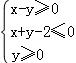
\includegraphics[width=.38\linewidth]{question-12-1.jpg}
\end{center}
\begin{choices}
  \item $3$
  \item $2\sqrt{2}$
  \item $\sqrt{5}$
  \item $2$
\end{choices}
\begin{solution}
\textbf{答案：}$A$

\textbf{分析：}如图：以$A$为原点，以$AB$，$AD$所在的直线为$x$，$y$轴建立如图所示的坐标系，先求出圆的标准方程，再设点$P$的坐标为$(\frac{2\sqrt{5}}{5}\cos\theta+1，\frac{2\sqrt{5}}{5}\sin\theta+2)$，根据$\overrightarrow{AP}=\lambda\overrightarrow{AB}+\mu\overrightarrow{AD}$，求出$\lambda$，$\mu$，根据三角函数的性质即可求出最值。

\textbf{详解：}如图：以$A$为原点，以$AB$，$AD$所在的直线为$x$，$y$轴建立如图所示的坐标系，则$A(0,0)$，$B(1,0)$，$D(0,2)$，$C(1,2)$。∵动点$P$在以点$C$为圆心且与$BD$相切的圆上，设圆的半径为$r$。∵$BC=2$，$CD=1$，∴$BD=\sqrt{BC^2+CD^2}=\sqrt{5}$。∴$\frac{1}{2}BC\cdot CD=\frac{1}{2}BD\cdot r$，∴$r=\frac{2\sqrt{5}}{5}$。∴圆的方程为$(x-1)^2+(y-2)^2=\frac{4}{5}$。设点$P$的坐标为$(\frac{2\sqrt{5}}{5}\cos\theta+1，\frac{2\sqrt{5}}{5}\sin\theta+2)$。∵$\overrightarrow{AP}=\lambda\overrightarrow{AB}+\mu\overrightarrow{AD}$，∴$(\frac{2\sqrt{5}}{5}\cos\theta+1，\frac{2\sqrt{5}}{5}\sin\theta+2)=\lambda(1,0)+\mu(0,2)=(\lambda,2\mu)$。∴$\frac{2\sqrt{5}}{5}\cos\theta+1=\lambda$，$\frac{2\sqrt{5}}{5}\sin\theta+2=2\mu$。∴$\lambda+\mu=\frac{\sqrt{5}}{5}\cos\theta+\frac{\sqrt{5}}{5}\sin\theta+2=\sin(\theta+\varphi)+2$，其中$\tan\varphi=2$。∵$-1\le\sin(\theta+\varphi)\le1$，∴$1\le\lambda+\mu\le3$，故$\lambda+\mu$的最大值为$3$。故选A。
\end{solution}
\end{question}

\section*{二、填空题}
本题共4小题，每小题5分，共20分。

\begin{question}[points=5]
若$x$，$y$满足约束条件$\begin{cases} x-y+1\ge 0 \\ x+y-3\le 0 \\ y\ge 0 \end{cases}$，则$z=3x-4y$的最小值为．
\fillin[{$-1$}]
\begin{solution}
\textbf{答案：}$-1$

\textbf{分析：}作出不等式组对应的平面区域，利用目标函数的几何意义，求目标函数$z=3x-4y$的最小值。

\textbf{详解：}由$z=3x-4y$，得$y=\frac{3}{4}x-\frac{z}{4}$，作出不等式对应的可行域（阴影部分），平移直线$y=\frac{3}{4}x-\frac{z}{4}$，由平移可知当直线$y=\frac{3}{4}x-\frac{z}{4}$经过点$B(1,1)$时，直线$y=\frac{3}{4}x-\frac{z}{4}$的截距最大，此时$z$取得最小值，将$B$的坐标代入$z=3x-4y=3-4=-1$，即目标函数$z=3x-4y$的最小值为$-1$。故答案为：$-1$。
\end{solution}
\end{question}

\begin{question}[points=5]
设等比数列$\{a_n\}$满足$a_1+a_2=-1$，$a_1-a_3=-3$，则$a_4=$．
\fillin[{$-8$}]
\begin{solution}
\textbf{答案：}$-8$

\textbf{分析：}设等比数列$\{a_n\}$的公比为$q$，由$a_1+a_2=-1$，$a_1-a_3=-3$，可得：$a_1(1+q)=-1$，$a_1(1-q^2)=-3$，解出即可得出。

\textbf{详解：}设等比数列$\{a_n\}$的公比为$q$，∵$a_1+a_2=-1$，$a_1-a_3=-3$，∴$a_1(1+q)=-1$，$a_1(1-q^2)=-3$，解得$a_1=1$，$q=-2$．则$a_4=(-2)^3=-8$。故答案为：$-8$。
\end{solution}
\end{question}

\begin{question}[points=5]
设函数$f(x)=\begin{cases} x+1, & x\le 0 \\ 2^x, & x>0 \end{cases}$，则满足$f(x)+f(x-\frac{1}{2})>1$的$x$的取值范围是．
\fillin[{$(-\frac{1}{4},+\infty)$}]
\begin{solution}
\textbf{答案：}$(-\frac{1}{4},+\infty)$

\textbf{分析：}根据分段函数的表达式，分别讨论$x$的取值范围，进行求解即可。

\textbf{详解：}若$x\le 0$，则$x-\frac{1}{2}\le -\frac{1}{2}$，则$f(x)+f(x-\frac{1}{2})>1$等价为$x+1+x-\frac{1}{2}+1>1$，即$2x>-\frac{1}{2}$，则$x>-\frac{1}{4}$，此时$-\frac{1}{4}<x\le 0$。当$x>0$时，$f(x)=2^x>1$，$x-\frac{1}{2}>-\frac{1}{2}$，当$x-\frac{1}{2}>0$即$x>\frac{1}{2}$时，满足$f(x)+f(x-\frac{1}{2})>1$恒成立。当$0\ge x-\frac{1}{2}>-\frac{1}{2}$，即$\frac{1}{2}\ge x>0$时，$f(x-\frac{1}{2})=x-\frac{1}{2}+1=x+\frac{1}{2}$，此时$f(x)+f(x-\frac{1}{2})>1$恒成立。综上$x>-\frac{1}{4}$。故答案为：$(-\frac{1}{4},+\infty)$。
\end{solution}
\end{question}

\begin{question}[points=5]
$a$，$b$为空间中两条互相垂直的直线，等腰直角三角形$ABC$的直角边$AC$所在直线与$a$，$b$都垂直，斜边$AB$以直线$AC$为旋转轴旋转，有下列结论：①当直线$AB$与$a$成$60^\circ$角时，$AB$与$b$成$30^\circ$角；②当直线$AB$与$a$成$60^\circ$角时，$AB$与$b$成$60^\circ$角；③直线$AB$与$a$所成角的最小值为$45^\circ$；④直线$AB$与$a$所成角的最小值为$60^\circ$；其中正确的是．（填写所有正确结论的编号）
\fillin[{$②③$}]
\begin{solution}
\textbf{答案：}$②③$

\textbf{分析：}由题意知，$a$、$b$、$AC$三条直线两两相互垂直，构建如图所示的边长为1的正方体，$|AC|=1$，$|AB|=\sqrt{2}$，斜边$AB$以直线$AC$为旋转轴，则$A$点保持不变，$B$点的运动轨迹是以$C$为圆心，1为半径的圆，以$C$坐标原点，以$CD$为$x$轴，$CB$为$y$轴，$CA$为$z$轴，建立空间直角坐标系，利用向量法能求出结果。

\textbf{详解：}由题意知，$a$、$b$、$AC$三条直线两两相互垂直，画出图形如图，不妨设图中所示正方体边长为1，故$|AC|=1$，$|AB|=\sqrt{2}$，斜边$AB$以直线$AC$为旋转轴，则$A$点保持不变，$B$点的运动轨迹是以$C$为圆心，1为半径的圆，以$C$坐标原点，以$CD$为$x$轴，$CB$为$y$轴，$CA$为$z$轴，建立空间直角坐标系，则$D(1,0,0)$，$A(0,0,1)$，直线$a$的方向单位向量$\overrightarrow{u}=(0,1,0)$，$|\overrightarrow{u}|=1$，直线$b$的方向单位向量$\overrightarrow{v}=(1,0,0)$，$|\overrightarrow{v}|=1$，设$B$点在运动过程中的坐标中的坐标$B'(\cos\theta,\sin\theta,0)$，其中$\theta$为$B'C$与$CD$的夹角，$\theta\in[0,2\pi)$，∴$AB'$在运动过程中的向量，$\overrightarrow{AB'}=(\cos\theta,\sin\theta,-1)$，$|\overrightarrow{AB'}|=\sqrt{2}$，设$\overrightarrow{AB'}$与$\overrightarrow{u}$所成夹角为$\alpha\in[0,\frac{\pi}{2}]$，则$\cos\alpha=\frac{|\overrightarrow{AB'}\cdot\overrightarrow{u}|}{|\overrightarrow{AB'}||\overrightarrow{u}|}=\frac{|\sin\theta|}{\sqrt{2}}\in[0,\frac{\sqrt{2}}{2}]$，∴$\alpha\in[\frac{\pi}{4},\frac{\pi}{2}]$，∴③正确，④错误。设$\overrightarrow{AB'}$与$\overrightarrow{v}$所成夹角为$\beta\in[0,\frac{\pi}{2}]$，$\cos\beta=\frac{|\overrightarrow{AB'}\cdot\overrightarrow{v}|}{|\overrightarrow{AB'}||\overrightarrow{v}|}=\frac{|\cos\theta|}{\sqrt{2}}$，当$\overrightarrow{AB'}$与$\overrightarrow{u}$夹角为$60^\circ$时，即$\alpha=60^\circ$，$\cos60^\circ=\frac{|\sin\theta|}{\sqrt{2}}=\frac{1}{2}$，∴$|\sin\theta|=\frac{\sqrt{2}}{2}$，∵$\cos^2\theta+\sin^2\theta=1$，∴$\cos\beta=\frac{|\cos\theta|}{\sqrt{2}}=\frac{1}{2}$，∵$\beta\in[0,\frac{\pi}{2}]$，∴$\beta=60^\circ$，此时$\overrightarrow{AB'}$与$\overrightarrow{v}$的夹角为$60^\circ$，∴②正确，①错误。故答案为：②③。
\end{solution}
\end{question}

\section*{三、解答题}
共70分。解答应写出文字说明、证明过程或演算步骤。第17~21题为必考题，每个试题考生都必须作答。第22、23题为选考题，考生根据要求作答。（一）必考题：60分。

\begin{question}[points=12]
$\triangle ABC$的内角$A$，$B$，$C$的对边分别为$a$，$b$，$c$，已知$\sin A+\sqrt{3}\cos A=0$，$a=2\sqrt{7}$，$b=2$．

（1）求$c$；

（2）设$D$为$BC$边上一点，且$AD\perp AC$，求$\triangle ABD$的面积．
\begin{solution}
\textbf{答案：}（1）$c=4$；（2）$\sqrt{3}$

\textbf{分析：}（1）先根据同角的三角函数的关系求出$A$，再根据余弦定理即可求出；（2）先根据夹角求出$\cos C$，求出$CD$的长，得到$S_{\triangle ABD}=\frac{1}{2}S_{\triangle ABC}$。

\textbf{详解：}解：（1）∵$\sin A+\sqrt{3}\cos A=0$，∴$\tan A=-\sqrt{3}$，∵$0<A<\pi$，∴$A=\frac{2\pi}{3}$。由余弦定理可得$a^2=b^2+c^2-2bc\cos A$，即$28=4+c^2-2\times2c\times(-\frac{1}{2})$，即$c^2+2c-24=0$，解得$c=-6$（舍去）或$c=4$，故$c=4$。
（2）∵$c^2=b^2+a^2-2ab\cos C$，∴$16=28+4-2\times2\sqrt{7}\times2\times\cos C$，∴$\cos C=\frac{2\sqrt{7}}{7}$，∴$CD=\frac{AC}{\cos C}=\frac{2}{\frac{2\sqrt{7}}{7}}=\sqrt{7}$。∴$CD=\frac{1}{2}BC$。∵$S_{\triangle ABC}=\frac{1}{2}AB\cdot AC\cdot\sin\angle BAC=\frac{1}{2}\times4\times2\times\frac{\sqrt{3}}{2}=2\sqrt{3}$，∴$S_{\triangle ABD}=\frac{1}{2}S_{\triangle ABC}=\sqrt{3}$。
\end{solution}
\end{question}

\begin{question}[points=12]
某超市计划按月订购一种酸奶，每天进货量相同，进货成本每瓶4元，售价每瓶6元，未售出的酸奶降价处理，以每瓶2元的价格当天全部处理完．根据往年销售经验，每天需求量与当天最高气温（单位：℃）有关．如果最高气温不低于25，需求量为500瓶；如果最高气温位于区间[20，25），需求量为300瓶；如果最高气温低于20，需求量为200瓶．为了确定六月份的订购计划，统计了前三年六月份各天的最高气温数据，得下面的频数分布表：



| 最高气温 | [10，15) | [15，20) | [20，25) | [25，30) | [30，35) | [35，40) |

|----------|----------|----------|----------|----------|----------|----------|

| 天数     | 2        | 16       | 36       | 25       | 7        | 4        |



以最高气温位于各区间的频率代替最高气温位于该区间的概率．

（1）求六月份这种酸奶一天的需求量$X$（单位：瓶）的分布列；

（2）设六月份一天销售这种酸奶的利润为$Y$（单位：元），当六月份这种酸奶一天的进货量$n$（单位：瓶）为多少时，$Y$的数学期望达到最大值？
\begin{solution}
\textbf{答案：}（1）分布列见解析；（2）$n=300$时，$EY$最大值为$520$元

\textbf{分析：}（1）由题意知$X$的可能取值为200，300，500，分别求出相应的概率，由此能求出$X$的分布列。（2）由题意知这种酸奶一天的需求量至多为500瓶，至少为200瓶，只需考虑$200\le n\le 500$，根据$300\le n\le 500$和$200\le n\le 300$分类讨论经，能得到当$n=300$时，$EY$最大值为520元。

\textbf{详解：}解：（1）由题意知$X$的可能取值为200，300，500，$P(X=200)=\frac{2+16}{90}=0.2$，$P(X=300)=\frac{36}{90}=0.4$，$P(X=500)=\frac{25+7+4}{90}=0.4$，∴$X$的分布列为：

| $X$ | 200 | 300 | 500 |
|-----|-----|-----|-----|
| $P$ | 0.2 | 0.4 | 0.4 |

（2）由题意知这种酸奶一天的需求量至多为500瓶，至少为200瓶，∴只需考虑$200\le n\le 500$，当$300\le n\le 500$时，若最高气温不低于25，则$Y=6n-4n=2n$；若最高气温位于区间[20，25），则$Y=6\times300+2(n-300)-4n=1200-2n$；若最高气温低于20，则$Y=6\times200+2(n-200)-4n=800-2n$，∴$EY=2n\times0.4+(1200-2n)\times0.4+(800-2n)\times0.2=640-0.4n$，当$200\le n\le 300$时，若最高气温不低于20，则$Y=6n-4n=2n$，若最高气温低于20，则$Y=6\times200+2(n-200)-4n=800-2n$，∴$EY=2n\times(0.4+0.4)+(800-2n)\times0.2=160+1.2n$．∴$n=300$时，$Y$的数学期望达到最大值，最大值为520元。
\end{solution}
\end{question}

\begin{question}[points=12]
如图，四面体$ABCD$中，$\triangle ABC$是正三角形，$\triangle ACD$是直角三角形，$\angle ABD=\angle CBD$，$AB=BD$．

（1）证明：平面$ACD\perp$平面$ABC$；

（2）过$AC$的平面交$BD$于点$E$，若平面$AEC$把四面体$ABCD$分成体积相等的两部分，求二面角$D-AE-C$的余弦值．

\begin{center}
  
\includegraphics[width=.38\linewidth]{question-19-1.jpg}
\end{center}
\begin{solution}
\textbf{答案：}（1）证明见解析；（2）$\frac{\sqrt{10}}{10}$

\textbf{分析：}（1）如图所示，取$AC$的中点$O$，连接$BO$，$OD$．$\triangle ABC$是等边三角形，可得$OB\perp AC$．由已知可得：$\triangle ABD\cong\triangle CBD$，$AD=CD$．$\triangle ACD$是直角三角形，可得$AC$是斜边，$\angle ADC=90^\circ$．可得$DO=\frac{1}{2}AC$．利用$DO^2+BO^2=AB^2=BD^2$．可得$OB\perp OD$．利用线面面面垂直的判定与性质定理即可证明．
（2）设点$D$，$B$到平面$ACE$的距离分别为$h_D$，$h_E$．则$\frac{h_D}{h_E}=\frac{VE-ACD}{VE-ABC}$．根据平面$AEC$把四面体$ABCD$分成体积相等的两部分，可得$\frac{VE-ACD}{VE-ABC}=\frac{VD-ACE}{VB-ACE}=1$，即点$E$是$BD$的中点．建立如图所示的空间直角坐标系．不妨取$AB=2$．利用法向量的夹角公式即可得出。

\textbf{详解：}（1）证明：如图所示，取$AC$的中点$O$，连接$BO$，$OD$．∵$\triangle ABC$是等边三角形，∴$OB\perp AC$．$\triangle ABD$与$\triangle CBD$中，$AB=BD=BC$，$\angle ABD=\angle CBD$，∴$\triangle ABD\cong\triangle CBD$，∴$AD=CD$．∵$\triangle ACD$是直角三角形，∴$AC$是斜边，∴$\angle ADC=90^\circ$．∴$DO=\frac{1}{2}AC$．∴$DO^2+BO^2=AB^2=BD^2$．∴$\angle BOD=90^\circ$．∴$OB\perp OD$．又$DO\cap AC=O$，∴$OB\perp$平面$ACD$．又$OB\subset$平面$ABC$，∴平面$ACD\perp$平面$ABC$．
（2）解：设点$D$，$B$到平面$ACE$的距离分别为$h_D$，$h_E$．则$\frac{h_D}{h_E}=\frac{V_{E-ACD}}{V_{E-ABC}}$．∵平面$AEC$把四面体$ABCD$分成体积相等的两部分，∴$\frac{V_{E-ACD}}{V_{E-ABC}}=\frac{V_{D-ACE}}{V_{B-ACE}}=1$．∴点$E$是$BD$的中点．建立如图所示的空间直角坐标系．不妨取$AB=2$．则$O(0,0,0)$，$A(1,0,0)$，$C(-1,0,0)$，$D(0,0,1)$，$B(0,\sqrt{3},0)$，$E(0,\frac{\sqrt{3}}{2},\frac{1}{2})$．$\overrightarrow{AD}=(-1,0,1)$，$\overrightarrow{AE}=(-1,\frac{\sqrt{3}}{2},\frac{1}{2})$，$\overrightarrow{AC}=(-2,0,0)$．设平面$ADE$的法向量为$\overrightarrow{n}=(x,y,z)$，则$\begin{cases} \overrightarrow{n}\cdot\overrightarrow{AD}=0 \\ \overrightarrow{n}\cdot\overrightarrow{AE}=0 \end{cases}$，即$\begin{cases} -x+z=0 \\ -x+\frac{\sqrt{3}}{2}y+\frac{1}{2}z=0 \end{cases}$，取$\overrightarrow{n}=(1,\frac{\sqrt{3}}{3},1)$．同理可得：平面$ACE$的法向量为$\overrightarrow{m}=(0,1,\sqrt{3})$．∴$\cos<\overrightarrow{n},\overrightarrow{m}>=\frac{\overrightarrow{n}\cdot\overrightarrow{m}}{|\overrightarrow{n}||\overrightarrow{m}|}=\frac{\frac{\sqrt{3}}{3}+\sqrt{3}}{\sqrt{1+\frac{1}{3}+1}\times\sqrt{1+3}}=\frac{\frac{4\sqrt{3}}{3}}{\sqrt{\frac{7}{3}}\times2}=\frac{\frac{4\sqrt{3}}{3}}{\frac{2\sqrt{21}}{3}}=\frac{2\sqrt{7}}{7}$．经检查，二面角$D-AE-C$的余弦值为$\frac{\sqrt{10}}{10}$。
\end{solution}
\end{question}

\begin{question}[points=12]
已知抛物线$C:y^2=2x$，过点$(2,0)$的直线$l$交$C$于$A$，$B$两点，圆$M$是以线段$AB$为直径的圆．

（1）证明：坐标原点$O$在圆$M$上；

（2）设圆$M$过点$P(4,-2)$，求直线$l$与圆$M$的方程．
\begin{solution}
\textbf{答案：}（1）证明见解析；（2）直线$l$的方程为$y=-2x+4$，圆$M$的方程$(x-\frac{9}{4})^2+(y+\frac{1}{2})^2=\frac{85}{16}$；或直线$l$的方程为$y=x-2$，圆$M$的方程为$(x-3)^2+(y-1)^2=10$

\textbf{分析：}（1）方法一：分类讨论，当直线斜率不存在时，求得$A$和$B$的坐标，由$\overrightarrow{OA}\cdot\overrightarrow{OB}=0$，则坐标原点$O$在圆$M$上；当直线$l$斜率存在，代入抛物线方程，利用韦达定理及向量数量积的可得$\overrightarrow{OA}\cdot\overrightarrow{OB}=0$，则坐标原点$O$在圆$M$上；
方法二：设直线$l$的方程$x=my+2$，代入抛物线方程，利用韦达定理及向量数量积的坐标运算，即可求得$\overrightarrow{OA}\cdot\overrightarrow{OB}=0$，则坐标原点$O$在圆$M$上；
（2）由题意可知：$\overrightarrow{AP}\cdot\overrightarrow{BP}=0$，根据向量数量积的坐标运算，即可求得$k$的值，求得$M$点坐标，则半径$r=|MP|$，即可求得圆的方程。

\textbf{详解：}解：（1）方法一：证明：当直线$l$的斜率不存在时，则$A(2,2)$，$B(2,-2)$，则$\overrightarrow{OA}=(2,2)$，$\overrightarrow{OB}=(2,-2)$，则$\overrightarrow{OA}\cdot\overrightarrow{OB}=0$，∴$\overrightarrow{OA}\perp\overrightarrow{OB}$，则坐标原点$O$在圆$M$上；当直线$l$的斜率存在，设直线$l$的方程$y=k(x-2)$，$A(x_1,y_1)$，$B(x_2,y_2)$，$\begin{cases} y=k(x-2) \\ y^2=2x \end{cases}$，整理得：$k^2x^2-(4k^2+2)x+4k^2=0$，则$x_1x_2=4$，$4x_1x_2=y_1^2y_2^2=(y_1y_2)^2$，由$y_1y_2<0$，则$y_1y_2=-4$，由$\overrightarrow{OA}\cdot\overrightarrow{OB}=x_1x_2+y_1y_2=0$，则$\overrightarrow{OA}\perp\overrightarrow{OB}$，则坐标原点$O$在圆$M$上，综上可知：坐标原点$O$在圆$M$上；
方法二：设直线$l$的方程$x=my+2$，$\begin{cases} x=my+2 \\ y^2=2x \end{cases}$，整理得：$y^2-2my-4=0$，$A(x_1,y_1)$，$B(x_2,y_2)$，则$y_1y_2=-4$，则$(y_1y_2)^2=4x_1x_2$，则$x_1x_2=4$，则$\overrightarrow{OA}\cdot\overrightarrow{OB}=x_1x_2+y_1y_2=0$，则$\overrightarrow{OA}\perp\overrightarrow{OB}$，则坐标原点$O$在圆$M$上，∴坐标原点$O$在圆$M$上；
（2）由（1）可知：$x_1x_2=4$，$x_1+x_2=\frac{4k^2+2}{k^2}$，$y_1+y_2=\frac{2}{k}$，$y_1y_2=-4$，圆$M$过点$P(4,-2)$，则$\overrightarrow{AP}=(4-x_1,-2-y_1)$，$\overrightarrow{BP}=(4-x_2,-2-y_2)$，由$\overrightarrow{AP}\cdot\overrightarrow{BP}=0$，则$(4-x_1)(4-x_2)+(-2-y_1)(-2-y_2)=0$，整理得：$k^2+k-2=0$，解得：$k=-2$，$k=1$，当$k=-2$时，直线$l$的方程为$y=-2x+4$，则$x_1+x_2=\frac{9}{4}$，$y_1+y_2=-1$，则$M(\frac{9}{4},-\frac{1}{2})$，半径为$r=|MP|=\sqrt{(4-\frac{9}{4})^2+(-2+\frac{1}{2})^2}=\frac{\sqrt{85}}{4}$，∴圆$M$的方程$(x-\frac{9}{4})^2+(y+\frac{1}{2})^2=\frac{85}{16}$．当直线斜率$k=1$时，直线$l$的方程为$y=x-2$，同理求得$M(3,1)$，则半径为$r=|MP|=\sqrt{(4-3)^2+(-2-1)^2}=\sqrt{10}$，∴圆$M$的方程为$(x-3)^2+(y-1)^2=10$，综上可知：直线$l$的方程为$y=-2x+4$，圆$M$的方程$(x-\frac{9}{4})^2+(y+\frac{1}{2})^2=\frac{85}{16}$，或直线$l$的方程为$y=x-2$，圆$M$的方程为$(x-3)^2+(y-1)^2=10$。
\end{solution}
\end{question}

\begin{question}[points=12]
已知函数$f(x)=x-1-a\ln x$．

（1）若$f(x)\ge 0$，求$a$的值；

（2）设$m$为整数，且对于任意正整数$n$，$(1+\frac{1}{2})(1+\frac{1}{2^2})\cdots(1+\frac{1}{2^n})<m$，求$m$的最小值．
\begin{solution}
\textbf{答案：}（1）$a=1$；（2）$m$的最小值为$3$

\textbf{分析：}（1）通过对函数$f(x)=x-1-a\ln x(x>0)$求导，分$a\le 0$、$a>0$两种情况考虑导函数$f'(x)$与$0$的大小关系可得结论；
（2）通过（1）可知$\ln x\le x-1$，进而取特殊值可知$\ln(1+\frac{1}{2^k})<\frac{1}{2^k}$，$k\in N^*$．一方面利用等比数列的求和公式放缩可知$(1+\frac{1}{2})(1+\frac{1}{2^2})\cdots(1+\frac{1}{2^n})<e$，另一方面可知$(1+\frac{1}{2})(1+\frac{1}{2^2})\cdots(1+\frac{1}{2^n})>2$，从而当$n\ge 3$时，$(1+\frac{1}{2})(1+\frac{1}{2^2})\cdots(1+\frac{1}{2^n})\in(2,e)$，比较可得结论。

\textbf{详解：}解：（1）因为函数$f(x)=x-1-a\ln x$，$x>0$，所以$f'(x)=1-\frac{a}{x}=\frac{x-a}{x}$，且$f(1)=0$．所以当$a\le 0$时$f'(x)>0$恒成立，此时$y=f(x)$在$(0,+\infty)$上单调递增，这与$f(x)\ge 0$矛盾；当$a>0$时令$f'(x)=0$，解得$x=a$，所以$y=f(x)$在$(0,a)$上单调递减，在$(a,+\infty)$上单调递增，即$f(x)_{\min}=f(a)$，若$a\neq 1$，则$f(a)<f(1)=0$，从而与$f(x)\ge 0$矛盾；所以$a=1$；
（2）由（1）可知当$a=1$时$f(x)=x-1-\ln x\ge 0$，即$\ln x\le x-1$，所以$\ln(x+1)\le x$当且仅当$x=0$时取等号，所以$\ln(1+\frac{1}{2^k})<\frac{1}{2^k}$，$k\in N^*$．$\ln(1+\frac{1}{2})+\ln(1+\frac{1}{2^2})+\cdots+\ln(1+\frac{1}{2^n})<\frac{1}{2}+\frac{1}{2^2}+\cdots+\frac{1}{2^n}=1-\frac{1}{2^n}<1$，即$(1+\frac{1}{2})(1+\frac{1}{2^2})\cdots(1+\frac{1}{2^n})<e$；因为$m$为整数，且对于任意正整数$n$，$(1+\frac{1}{2})(1+\frac{1}{2^2})\cdots(1+\frac{1}{2^n})<m$成立，当$n=3$时，不等式左边大于$2$，所以$m$的最小值为$3$。
\end{solution}
\end{question}

\section*{（二）选考题}
共10分。请考生在第22、23题中任选一题作答，如果多做，则按所做的第一题计分。[选修4-4：坐标系与参数方程]

\begin{question}[points=10]
在直角坐标系$xOy$中，直线$l_1$的参数方程为$\begin{cases} x=2+t \\ y=kt \end{cases}$（$t$为参数），直线$l_2$的参数方程为$\begin{cases} x=-2+m \\ y=\frac{m}{k} \end{cases}$（$m$为参数）．设$l_1$与$l_2$的交点为$P$，当$k$变化时，$P$的轨迹为曲线$C$．

（1）写出$C$的普通方程；

（2）以坐标原点为极点，$x$轴正半轴为极轴建立极坐标系，设$l_3:\rho(\cos\theta+\sin\theta)-\sqrt{2}=0$，$M$为$l_3$与$C$的交点，求$M$的极径．
\begin{solution}
\textbf{答案：}（1）$x^2-y^2=4(x\neq 2$且$y\neq 0)$；（2）$\sqrt{5}$

\textbf{分析：}解：（1）分别消掉参数$t$与$m$可得直线$l_1$与直线$l_2$的普通方程为$y=k(x-2)$①与$x=-2+ky$②；联立①②，消去$k$可得$C$的普通方程为$x^2-y^2=4$；
（2）将$l_3$的极坐标方程为$\rho(\cos\theta+\sin\theta)-\sqrt{2}=0$化为普通方程：$x+y-\sqrt{2}=0$，再与曲线$C$的方程联立，可得$\begin{cases} x=\frac{3\sqrt{2}}{2} \\ y=-\frac{\sqrt{2}}{2} \end{cases}$，即可求得$l_3$与$C$的交点$M$的极径为$\rho=\sqrt{5}$。

\textbf{详解：}解：（1）∵直线$l_1$的参数方程为$\begin{cases} x=2+t \\ y=kt \end{cases}$（$t$为参数），∴消掉参数$t$得：直线$l_1$的普通方程为：$y=k(x-2)$①；又直线$l_2$的参数方程为$\begin{cases} x=-2+m \\ y=\frac{m}{k} \end{cases}$（$m$为参数），同理可得，直线$l_2$的普通方程为：$x=-2+ky$②；联立①②，消去$k$得：$x^2-y^2=4$，即$C$的普通方程为$x^2-y^2=4(x\neq 2$且$y\neq 0)$；
（2）∵$l_3$的极坐标方程为$\rho(\cos\theta+\sin\theta)-\sqrt{2}=0$，∴其普通方程为：$x+y-\sqrt{2}=0$，联立$\begin{cases} x+y-\sqrt{2}=0 \\ x^2-y^2=4 \end{cases}$得：$\begin{cases} x=\frac{3\sqrt{2}}{2} \\ y=-\frac{\sqrt{2}}{2} \end{cases}$，∴$\rho^2=x^2+y^2=\frac{9}{2}+\frac{1}{2}=5$．∴$l_3$与$C$的交点$M$的极径为$\rho=\sqrt{5}$。
\end{solution}
\end{question}

\begin{question}[points=10]
[选修4-5：不等式选讲]

已知函数$f(x)=|x+1|-|x-2|$．

（1）求不等式$f(x)\ge 1$的解集；

（2）若不等式$f(x)\ge x^2-x+m$的解集非空，求$m$的取值范围．
\begin{solution}
\textbf{答案：}（1）$\{x|x\ge 1\}$；（2）$(-\infty,\frac{5}{4}]$

\textbf{分析：}（1）由于$f(x)=|x+1|-|x-2|=\begin{cases} -3, & x\le -1 \\ 2x-1, & -1<x<2 \\ 3, & x\ge 2 \end{cases}$，解不等式$f(x)\ge 1$可分$-1\le x\le 2$与$x>2$两类讨论即可解得不等式$f(x)\ge 1$的解集；
（2）依题意可得$m\le [f(x)-x^2+x]_{max}$，设$g(x)=f(x)-x^2+x$，分$x\le 1$、$-1<x<2$、$x\ge 2$三类讨论，可求得$g(x)_{max}=\frac{5}{4}$，从而可得$m$的取值范围。

\textbf{详解：}解：（1）∵$f(x)=|x+1|-|x-2|=\begin{cases} -3, & x\le -1 \\ 2x-1, & -1<x<2 \\ 3, & x\ge 2 \end{cases}$，$f(x)\ge 1$，∴当$-1\le x\le 2$时，$2x-1\ge 1$，解得$1\le x\le 2$；当$x>2$时，$3\ge 1$恒成立，故$x>2$；综上，不等式$f(x)\ge 1$的解集为$\{x|x\ge 1\}$．
（2）原式等价于存在$x\in R$使得$f(x)-x^2+x\ge m$成立，即$m\le [f(x)-x^2+x]_{max}$，设$g(x)=f(x)-x^2+x$．由（1）知，$g(x)=\begin{cases} -x^2+x-3, & x\le -1 \\ -x^2+3x-1, & -1<x<2 \\ -x^2+x+3, & x\ge 2 \end{cases}$，当$x\le -1$时，$g(x)=-x^2+x-3$，其开口向下，对称轴方程为$x=\frac{1}{2}>-1$，∴$g(x)\le g(-1)=-1-1-3=-5$；当$-1<x<2$时，$g(x)=-x^2+3x-1$，其开口向下，对称轴方程为$x=\frac{3}{2}\in(-1,2)$，∴$g(x)\le g(\frac{3}{2})=-\frac{9}{4}+\frac{9}{2}-1=\frac{5}{4}$；当$x\ge 2$时，$g(x)=-x^2+x+3$，其开口向下，对称轴方程为$x=\frac{1}{2}<2$，∴$g(x)\le g(2)=-4+2+3=1$；综上，$g(x)_{max}=\frac{5}{4}$，∴$m$的取值范围为$(-\infty,\frac{5}{4}]$。
\end{solution}
\end{question}

